% ---------------------------- Preamble starts here ----------------------------

\documentclass[aspectratio=169]{beamer} %Remove [aspectratio=169] to get non-wide 4:3 slide aspect ratio

%-----------------------------------------------
% --- Set beamer theme
\usetheme{Metropolis}
\setbeamertemplate{footline}{}				% Remove automatic footer
\setbeamertemplate{navigation symbols}{}	% Comment this line to display navigation symbols

%-----------------------------------------------
% Load i2i symbol
\addtobeamertemplate{frametitle}{}{%
\begin{textblock*}{\linewidth}(0cm,7.4cm) % Replace with (0cm, 8cm) if using non-wide slide aspect
	
\includegraphics[width=\linewidth]{../../Common-Resources/img/Footer.png}
\end{textblock*}}

%-----------------------------------------------
% --- Load packages
\usepackage{textpos}		% To align objects correctly
\usepackage{multicol}		% To right in multiple columns
\usepackage{color}			% To color text

%-----------------------------------------------
% --- Include link to last commit
\usepackage{xstring}
\usepackage{catchfile}

%Set this user input
\newcommand{\gitfolder}{../../../.git} %relative path to .git folder from .tex doc
\newcommand{\reponame}{worldbank/dime-github-trainings} % Name of account and repo be set in URL

%Based on this https://tex.stackexchange.com/questions/455396/how-to-include-the-current-git-commit-id-and-branch-in-my-document
\CatchFileDef{\headfull}{\gitfolder/HEAD.}{} 				%Get path to head file for checked out branch
\StrGobbleRight{\headfull}{1}[\head]						%Remove end of line character
\StrBehind[2]{\head}{/}[\branch]							%Parse out the path only
\CatchFileDef{\commit}{\gitfolder/refs/heads/\branch.}{}	%Get the content of the branch head
\StrGobbleRight{\commit}{1}[\commithash]					%Remove end of line characted

%Build the URL to this commit based on the information we now have
\newcommand{\commiturl}{\url{https://github.com/\reponame/commit/\commithash}}

%-----------------------------------------------
% --- Add your information here
\title{GitHub - Pull Request training}
\author{DIME Analytics}
\institute{DIME - The World Bank - \trainingURL{https://www.worldbank.org/en/research/dime}}
\date{\today}

\newcommand{\trainingURL}[1]{{\color{blue}\url{#1}}}

\newcommand{\traininerUsername}{kbjarkefur}
\newcommand{\repoName}{\traininerUsername/lyrics}
\newcommand{\trainingRepoURL}[1]{\trainingURL{github.com/\repoName #1}}
\newcommand{\trainerEmail}{\trainingURL{kbjarkefur@worldbank.org} }


% ---------------------------- Preamble ends here ----------------------------

\begin{document}

\begin{frame}

\includegraphics[width=\textwidth]{../../Common-Resources/img/Header.png}
\vspace{-0.2cm}
\titlepage 	 % Opening slide, prints inform
\end{frame}

\section{Background}


\begin{frame}
\frametitle{What this training is and isn't}

Get more out of the "branch-PR-merge" cycle.

\begin{itemize}
	\item Part 1 - Best practices for the \textit{branch-PR-merge} cycle 
	\item Part 2 - How to fit the \textit{branch-PR-merge} cycle into your workflow
\end{itemize}


\end{frame}

\begin{frame}
	\frametitle{Who is this training for}
	
	You are comfortable branching, committing and merging in Git/GitHub
	
	But you wonder if you are doing it in the best away and if you are unaware of some 

\end{frame}

\section{Part 1: \newline Best practices for the branch-PR-merge cycle}

\begin{frame}
\frametitle{The branch-PR-merge cycle}

	\begin{columns}[c]
	
		\column{.35\textwidth} % Left column and width
		\large The branch-PR-merge cycle 
		\vspace{.7cm}\newline
		\large Complete this cycle for \textbf{all tasks}
		\vspace{.7cm}\newline
		\large We will go over all steps but focus today on the \textbf{work stage}	

		\column{.65\textwidth} % Right column and width
		\vspace{-.75cm}
		\begin{figure}
			\centering
			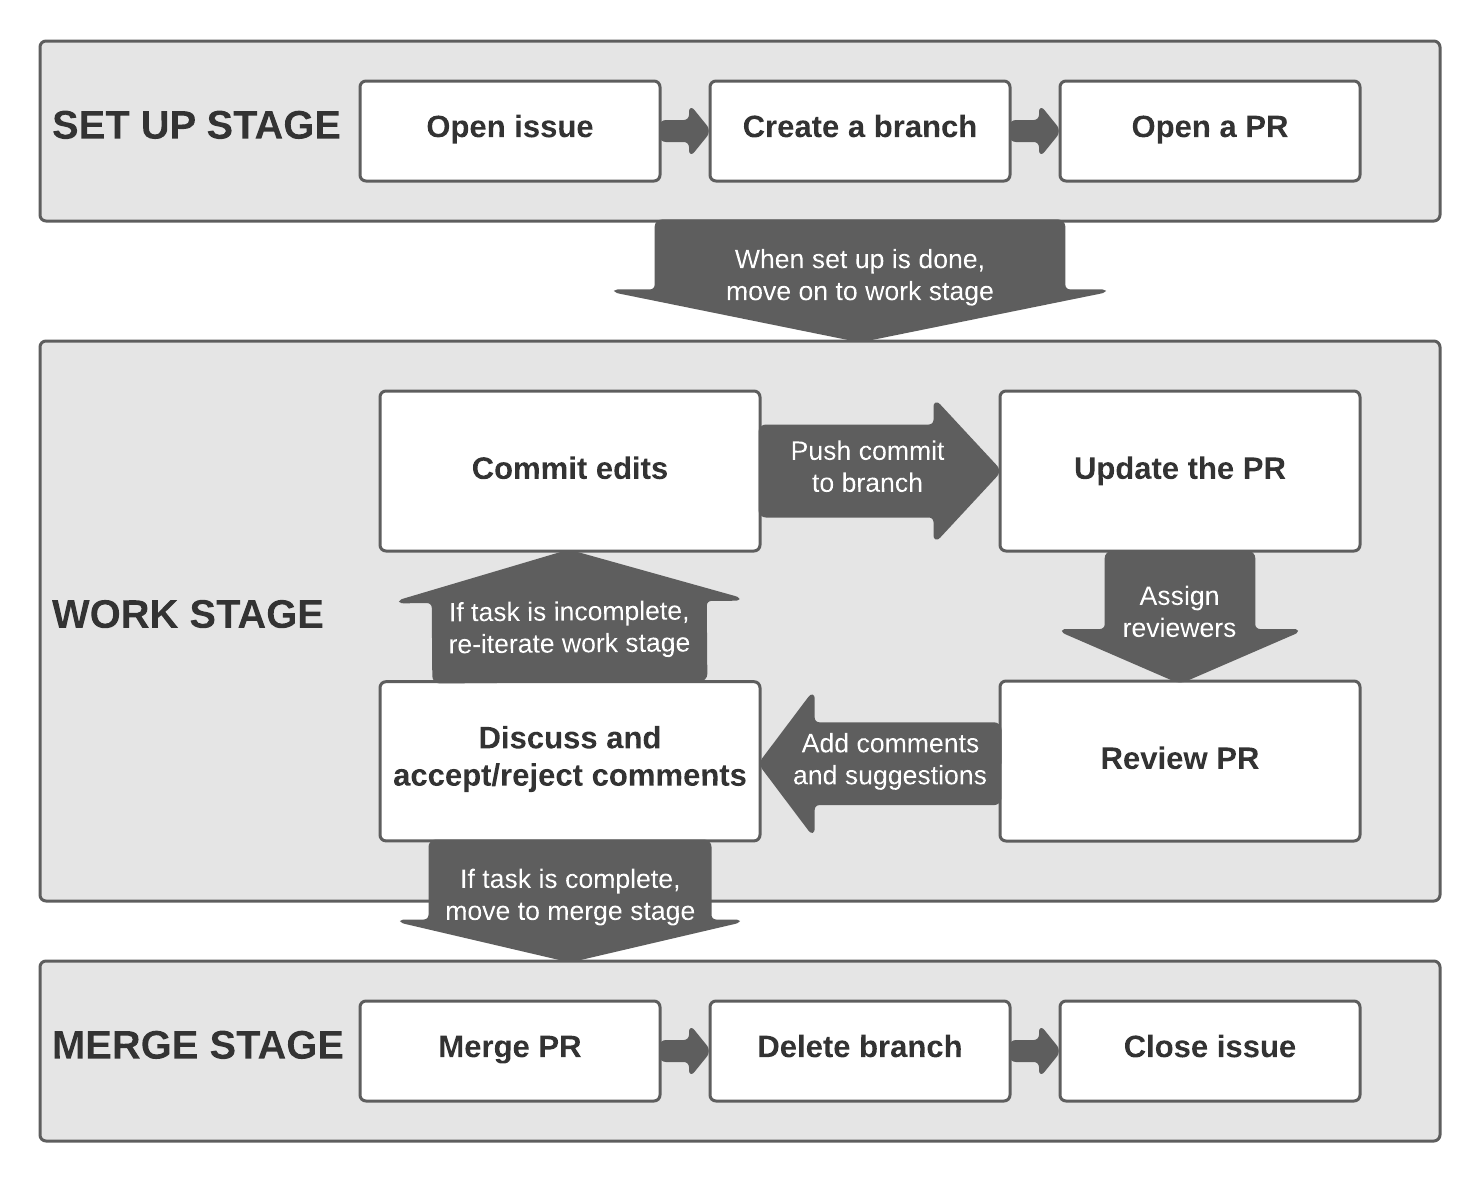
\includegraphics[width=\textwidth]{./img/branch-pr-merge-cycle.png}
		\end{figure}
		
	\end{columns}
\end{frame}


\begin{frame}
	\frametitle{Stage: The set up stage}
	\begin{columns}[c]
		
		\column{.35\textwidth} % Left column and width
		\begin{itemize}
			\setlength\itemsep{1em}
			\item Document the task you will work on
			\item Create a space in your repo where to work on the task
		\end{itemize}
		
		\column{.65\textwidth} % Right column and width
		\vspace{-.75cm}
		\begin{figure}
			\centering
			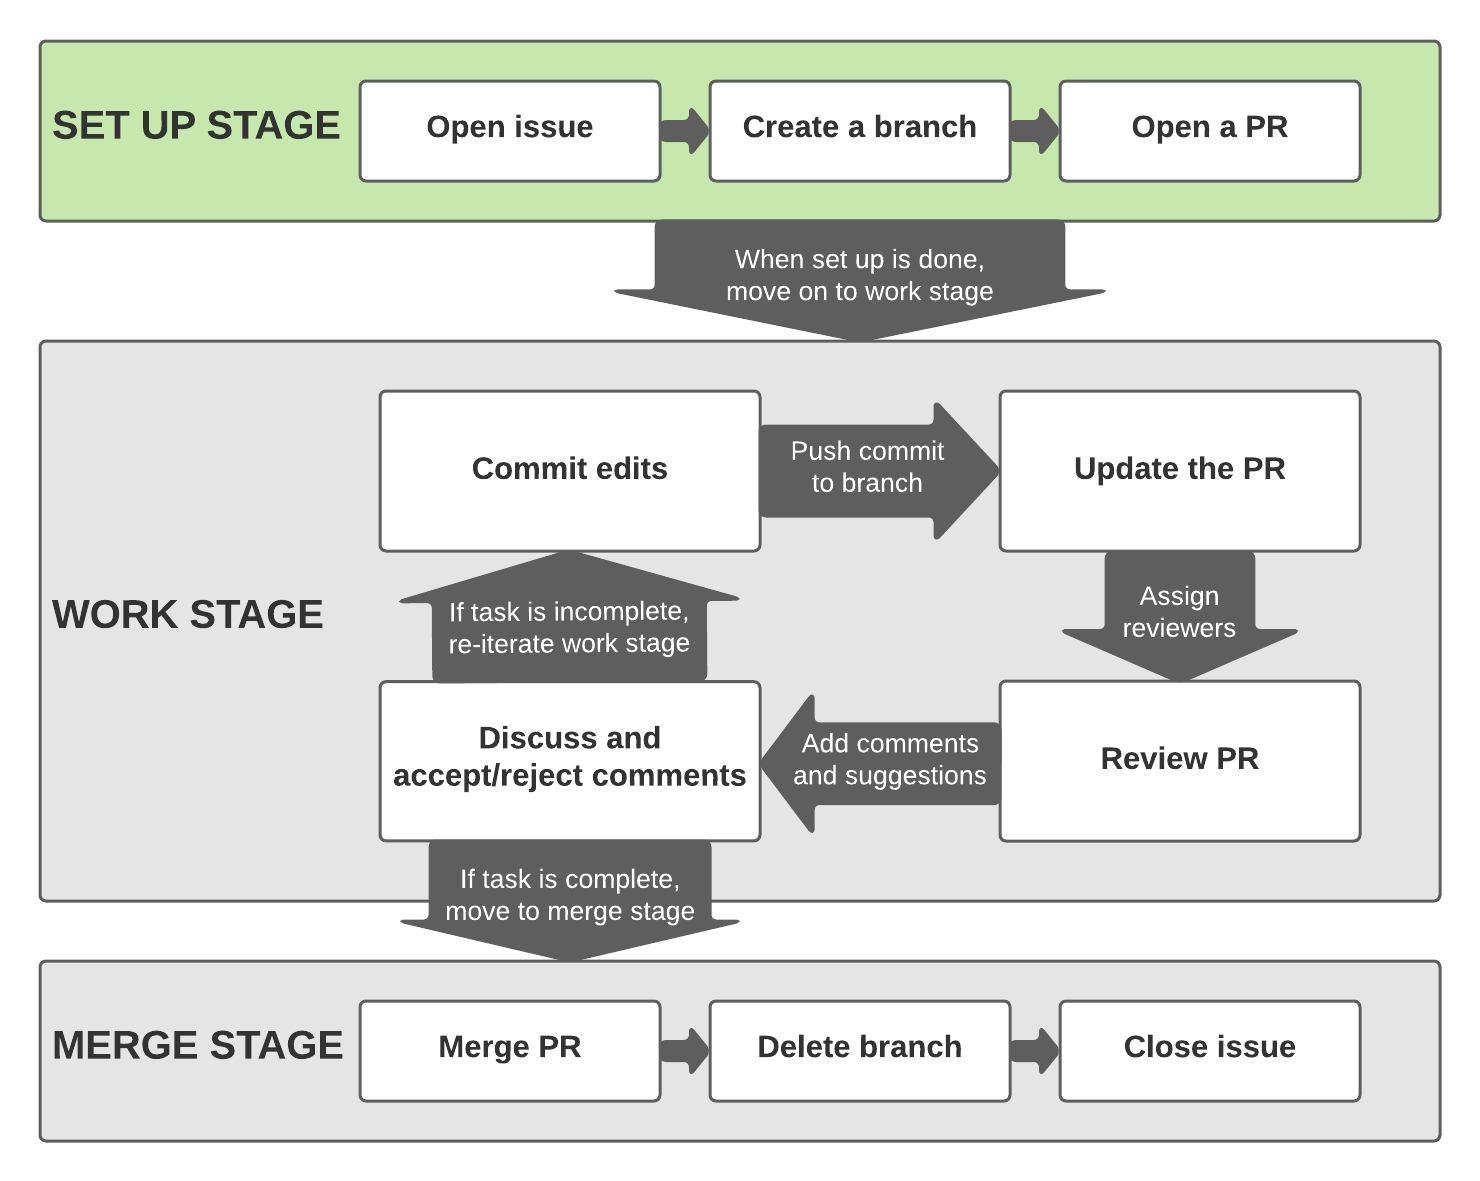
\includegraphics[width=\textwidth]{./img/branch-pr-merge-cycle-S1.png}
		\end{figure}
		
	\end{columns}
\end{frame}


\begin{frame}
	\frametitle{Step: Create an issue}
	\begin{columns}[c]
		
		\column{.35\textwidth} % Left column and width
		\begin{itemize}
			\setlength\itemsep{1em}
			\item Issues is a great way to document what tasks needs to be done
			\item Allows other team members to provide input on how to solve something
			\item Not needed if the task will be done immediately
		\end{itemize}
		
		\column{.65\textwidth} % Right column and width
		\vspace{-.75cm}
		\begin{figure}
			\centering
			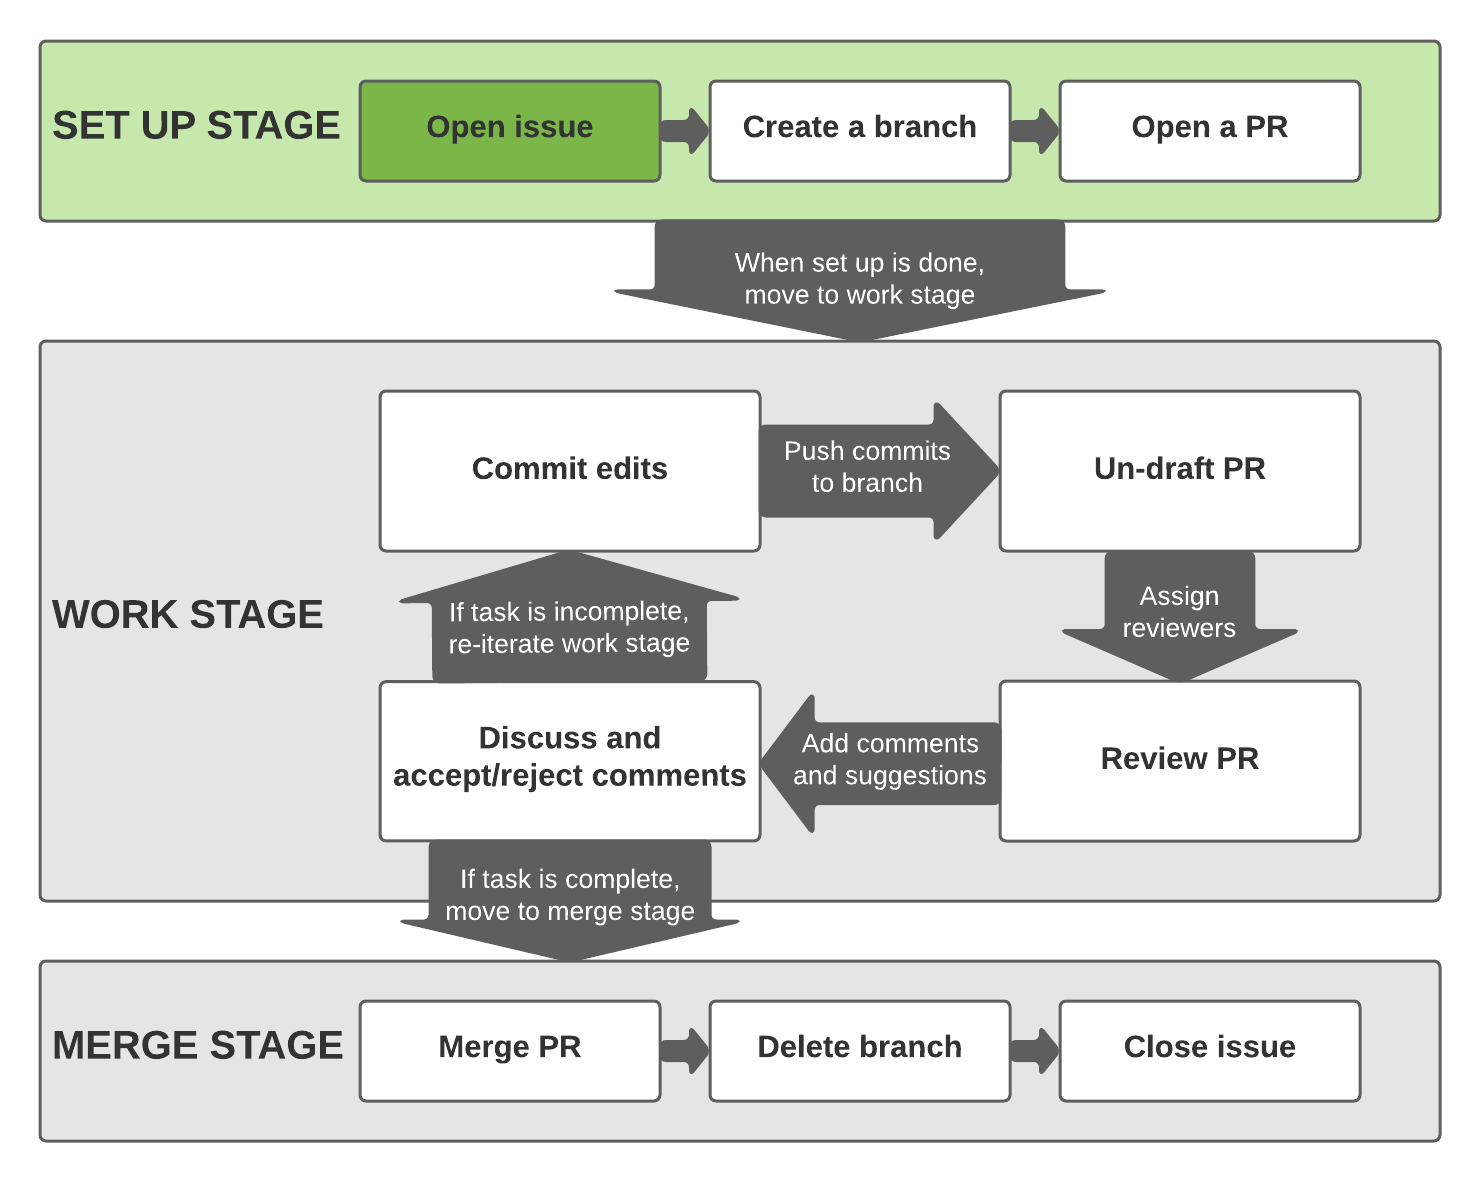
\includegraphics[width=\textwidth]{./img/branch-pr-merge-cycle-S1-1.png}
		\end{figure}
		
	\end{columns}
\end{frame}

\begin{frame}
	\frametitle{Create an issue}
	\begin{columns}[c]

		\column{.55\textwidth} % Right column and width
		\vspace{-.5cm}
		\begin{figure}
			\centering
			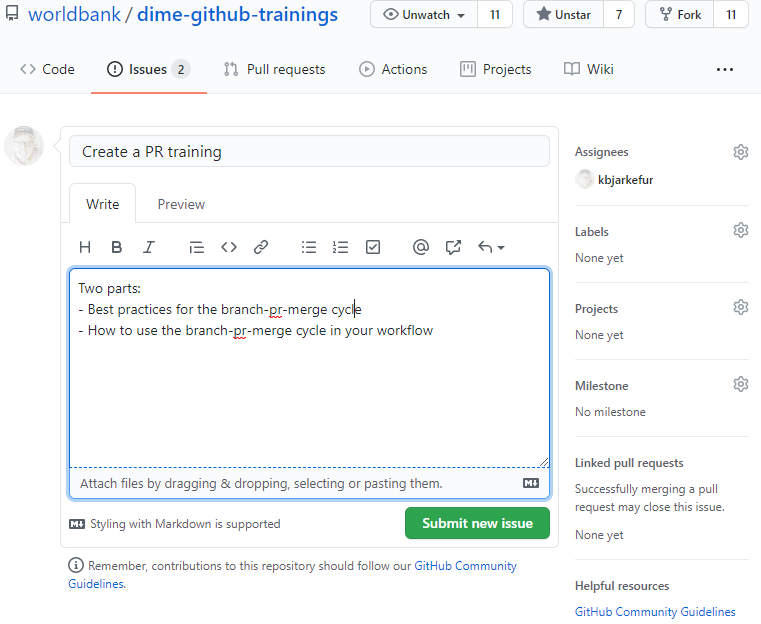
\includegraphics[width=\textwidth]{./img/create-issue-1.png}
		\end{figure}
		
		\column{.45\textwidth} % Left column and width
		
		\begin{itemize}
			\setlength\itemsep{.5em}
			\item Click the issues tab and then \texttt{New Issue}
			\item Document the task and/or ask the rest of the team of input
			\item Assign yourself of someone - add labels
			\item A far superior way to document tasks compared to emails or in-person meetings
		\end{itemize}
			
	\end{columns}	
\end{frame}

\begin{frame}
	\frametitle{Browse an issue}
	\begin{columns}[c]
		
		\column{.55\textwidth} % Right column and width
		\vspace{-.5cm}
		\begin{figure}
			\centering
			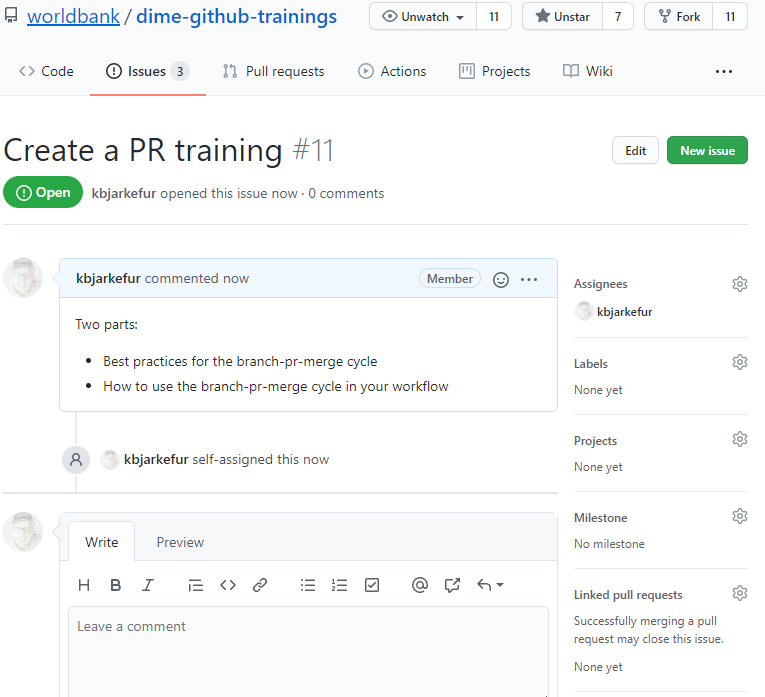
\includegraphics[width=\textwidth]{./img/create-issue-2.png}
		\end{figure}
		
		\column{.45\textwidth} % Left column and width
		
		\begin{itemize}
			\setlength\itemsep{1em}
			\item Take note of issue number - can also be found in URL
			\item Anyone can use comment field to provide input
			\item You can update assignee and/or labels
			\item Even when closed, this issue may be browsed by future team members
		\end{itemize}
		
	\end{columns}	
\end{frame}

\begin{frame}
	\frametitle{Create a branch}
	\begin{columns}[c]
		
		\column{.35\textwidth} % Left column and width
		\begin{itemize}
			\setlength\itemsep{1em}
			\item Create branch on GitHub.com
			\item Name it after the task and suffix name with issue number
			\item For example: \texttt{pr-training-11}
		\end{itemize}
		
		\column{.65\textwidth} % Right column and width
		\vspace{-.75cm}
		\begin{figure}
			\centering
			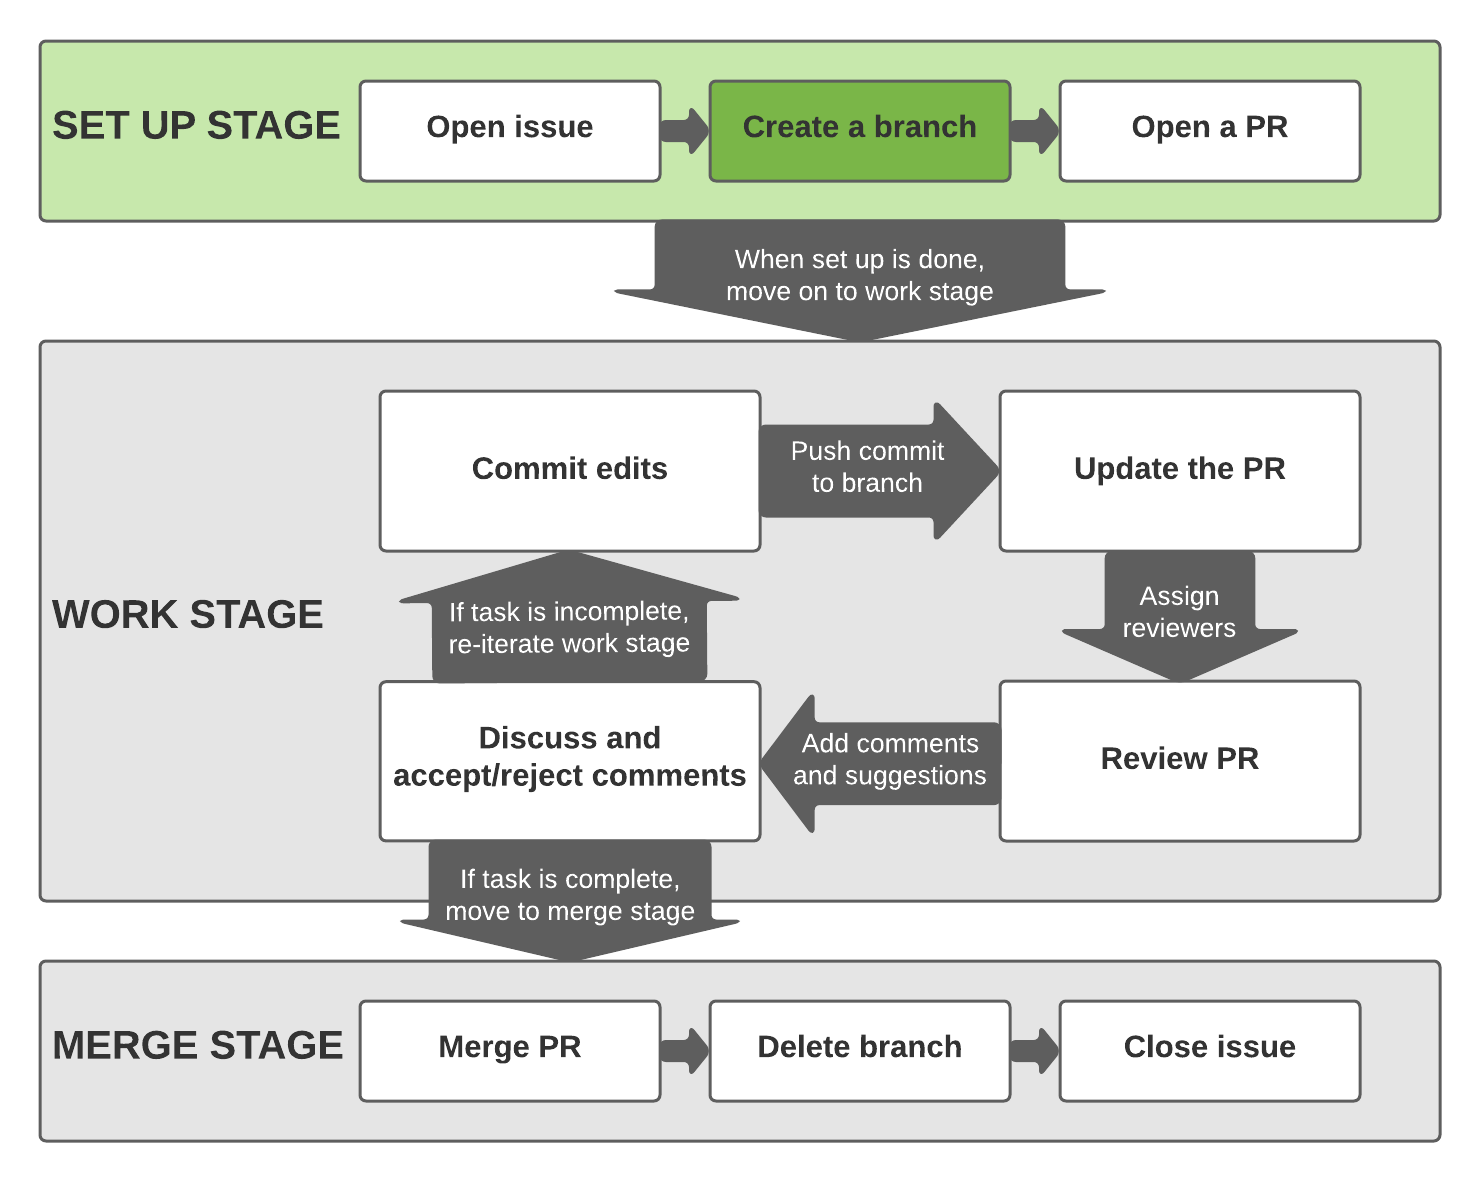
\includegraphics[width=\textwidth]{./img/branch-pr-merge-cycle-S1-2.png}
		\end{figure}
		
	\end{columns}
\end{frame}

\begin{frame}
	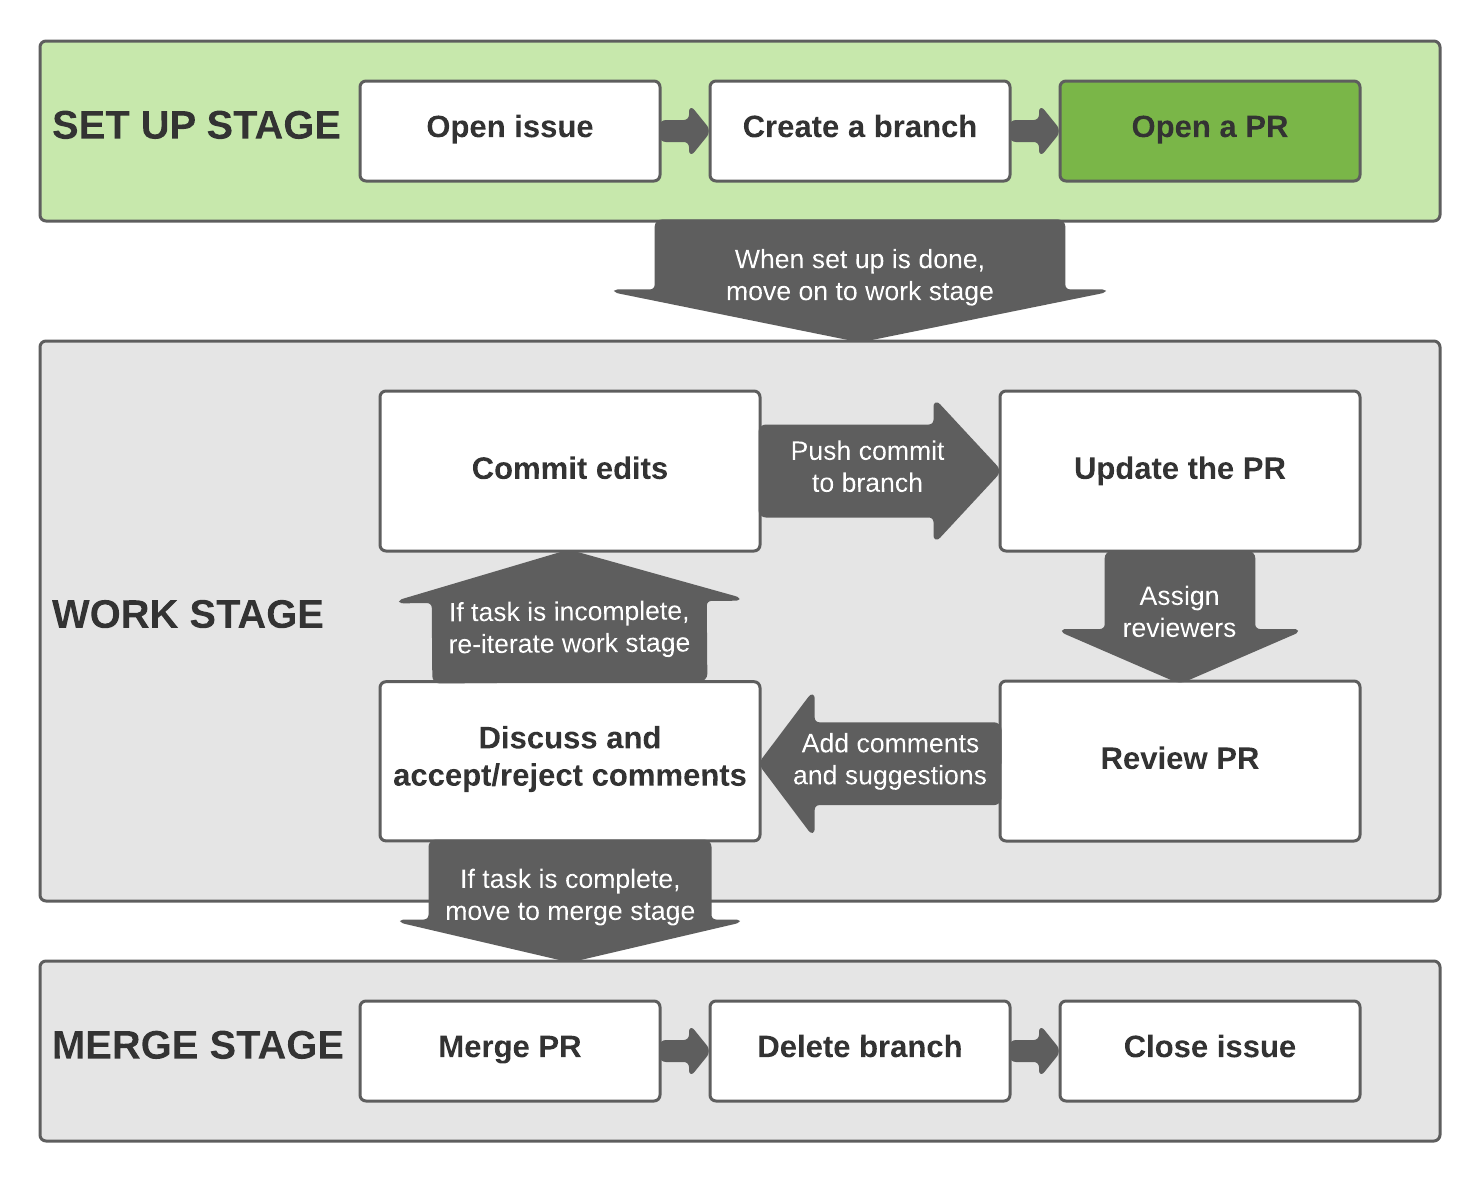
\includegraphics[width=\textwidth]{./img/branch-pr-merge-cycle-S1-3.png}
\end{frame}

\begin{frame}
	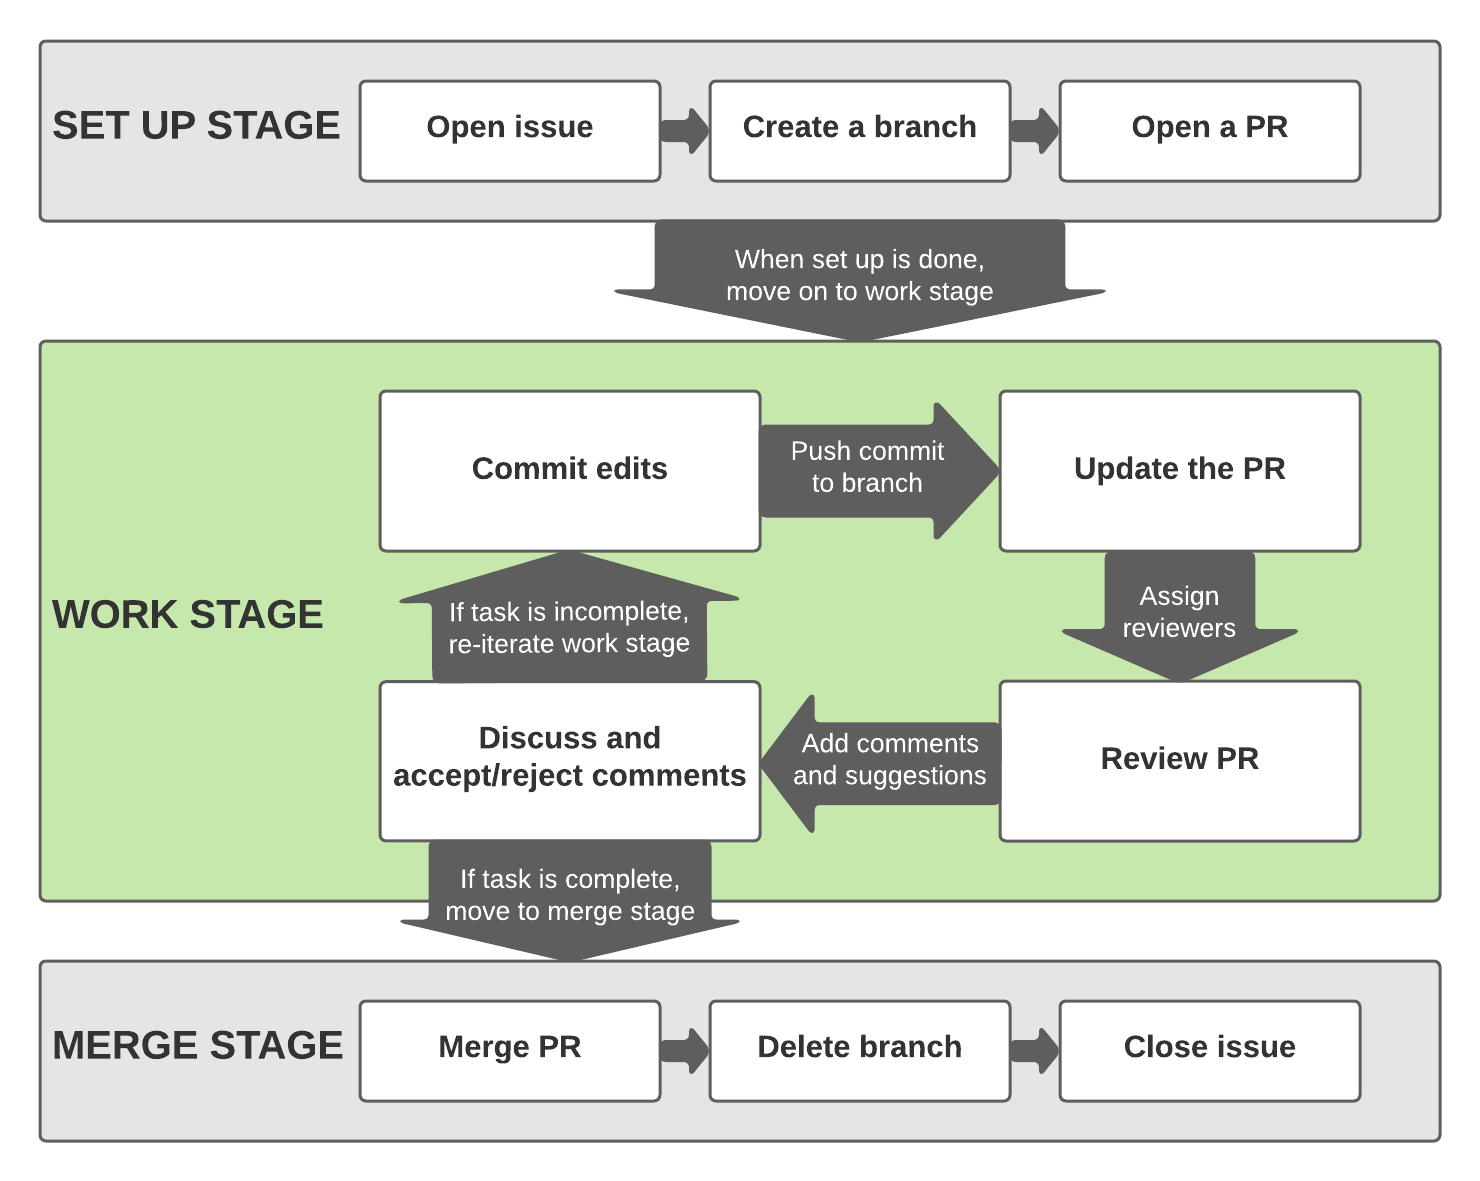
\includegraphics[width=\textwidth]{./img/branch-pr-merge-cycle-S2.png}
\end{frame}

\begin{frame}
	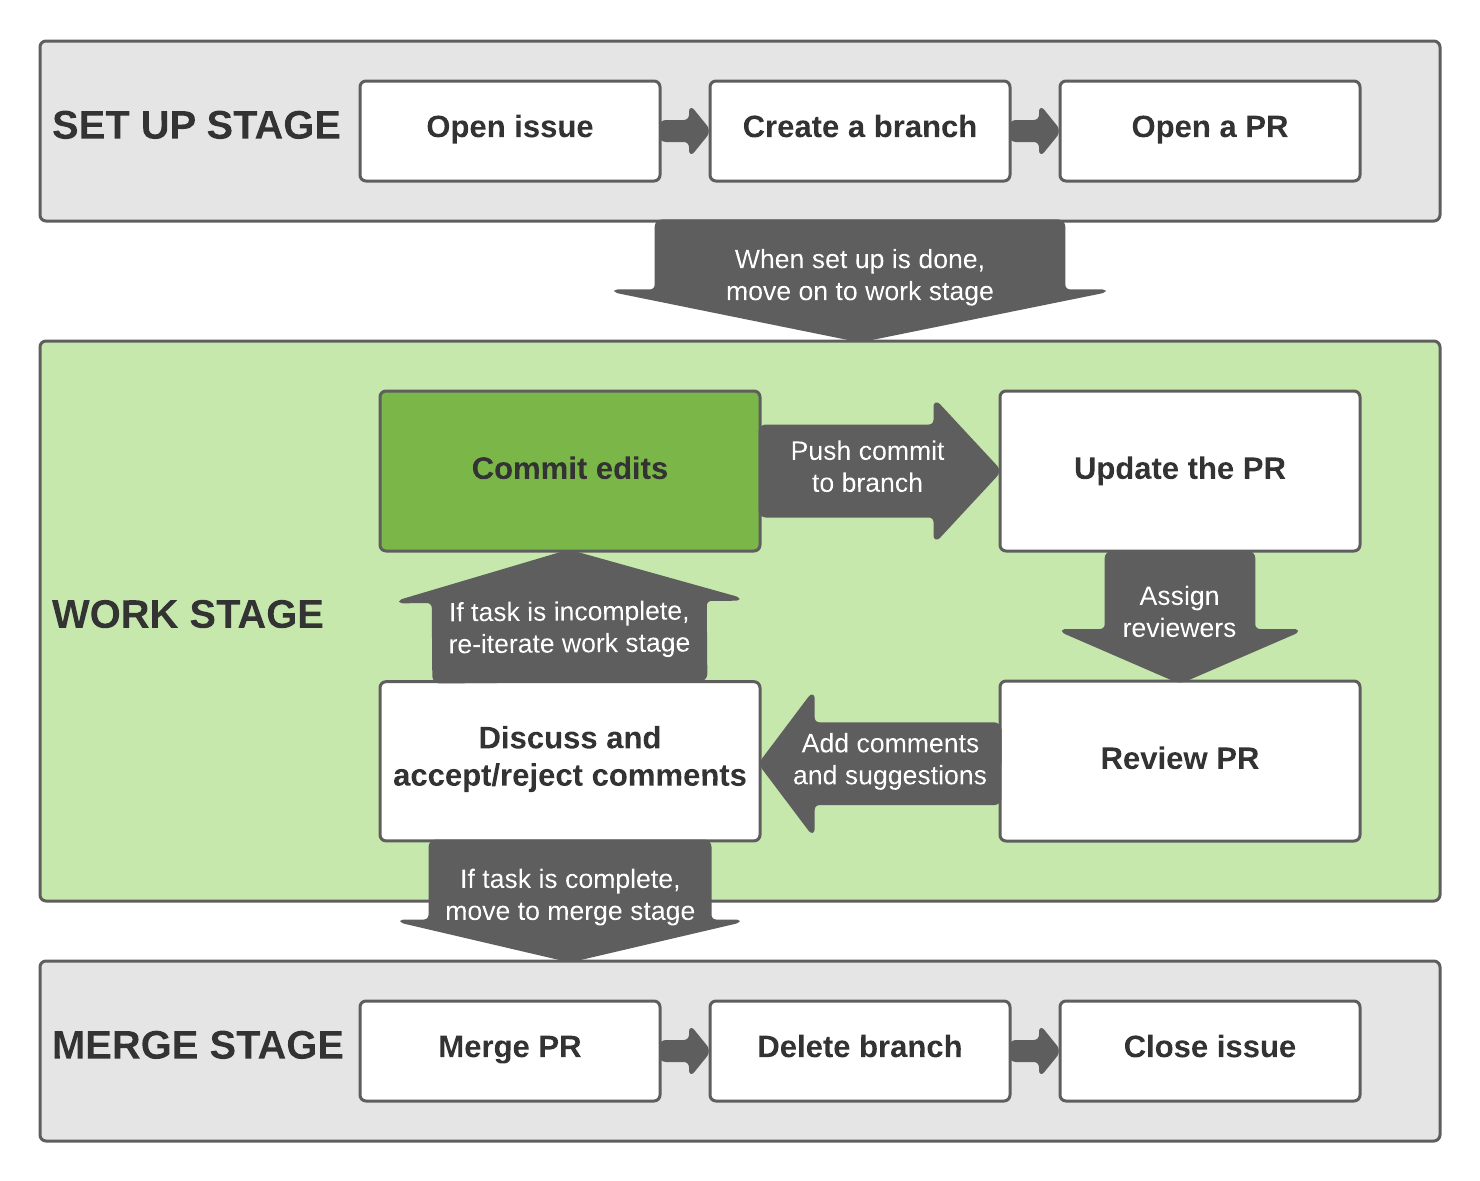
\includegraphics[width=\textwidth]{./img/branch-pr-merge-cycle-S2-1.png}
\end{frame}

\begin{frame}
	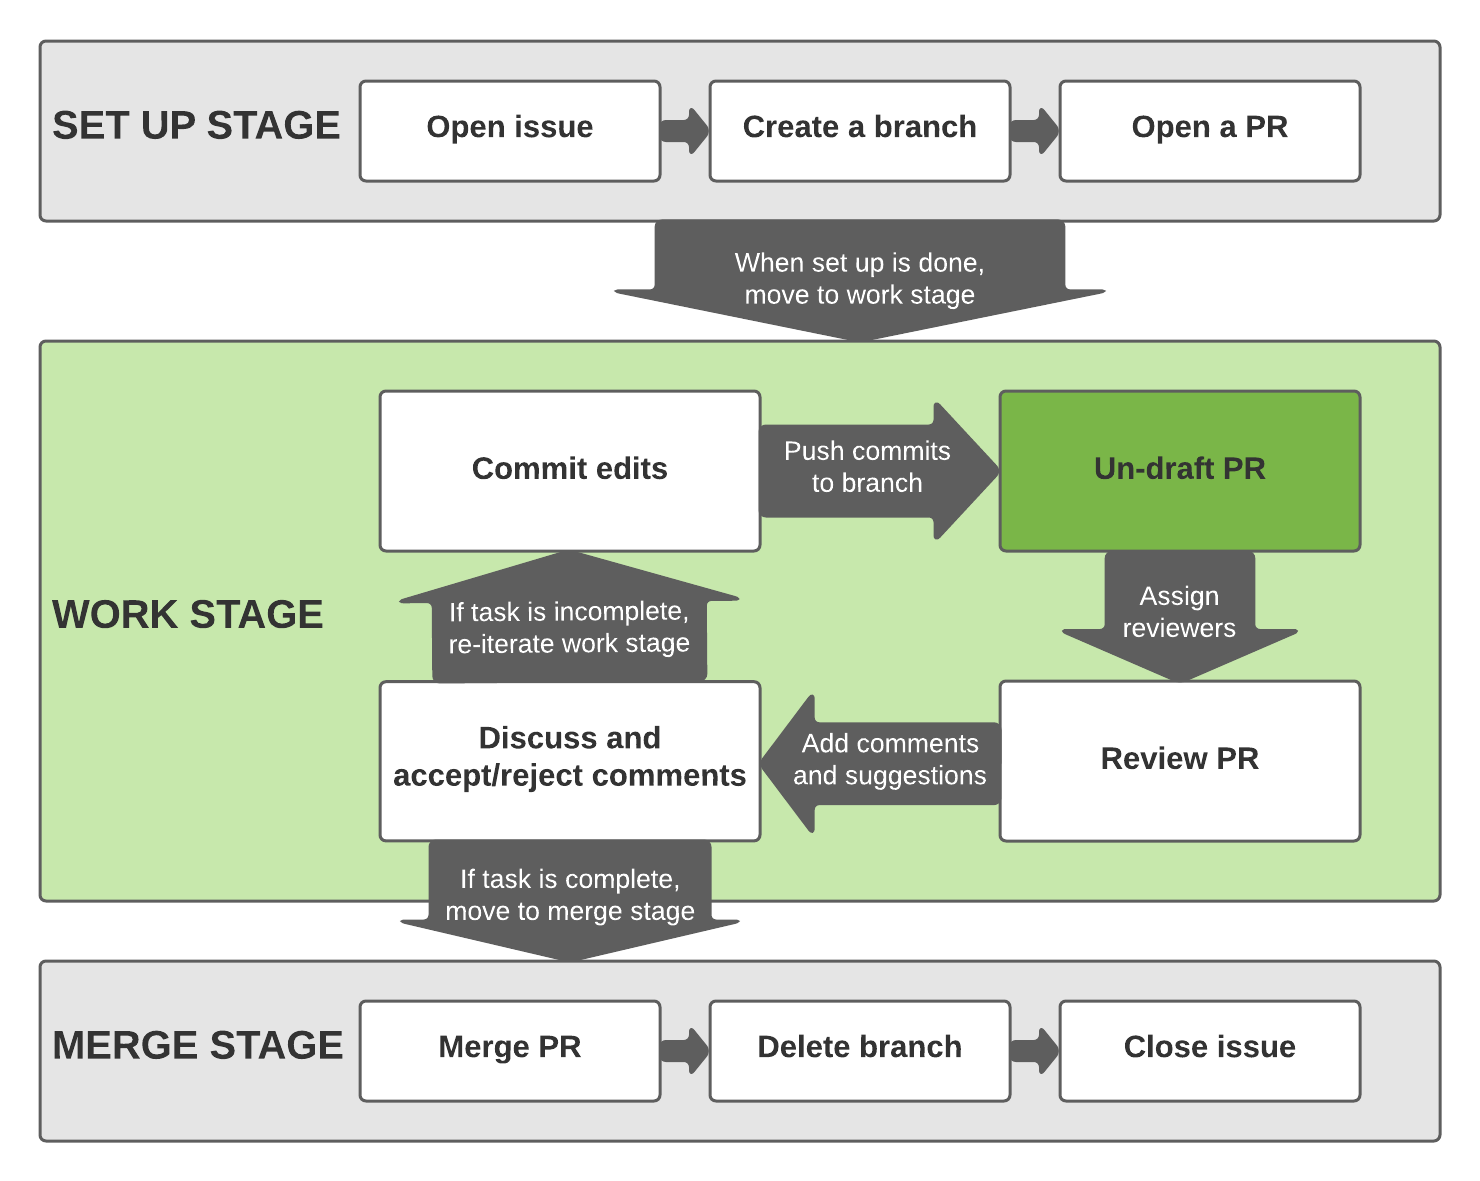
\includegraphics[width=\textwidth]{./img/branch-pr-merge-cycle-S2-2.png}
\end{frame}

\begin{frame}
	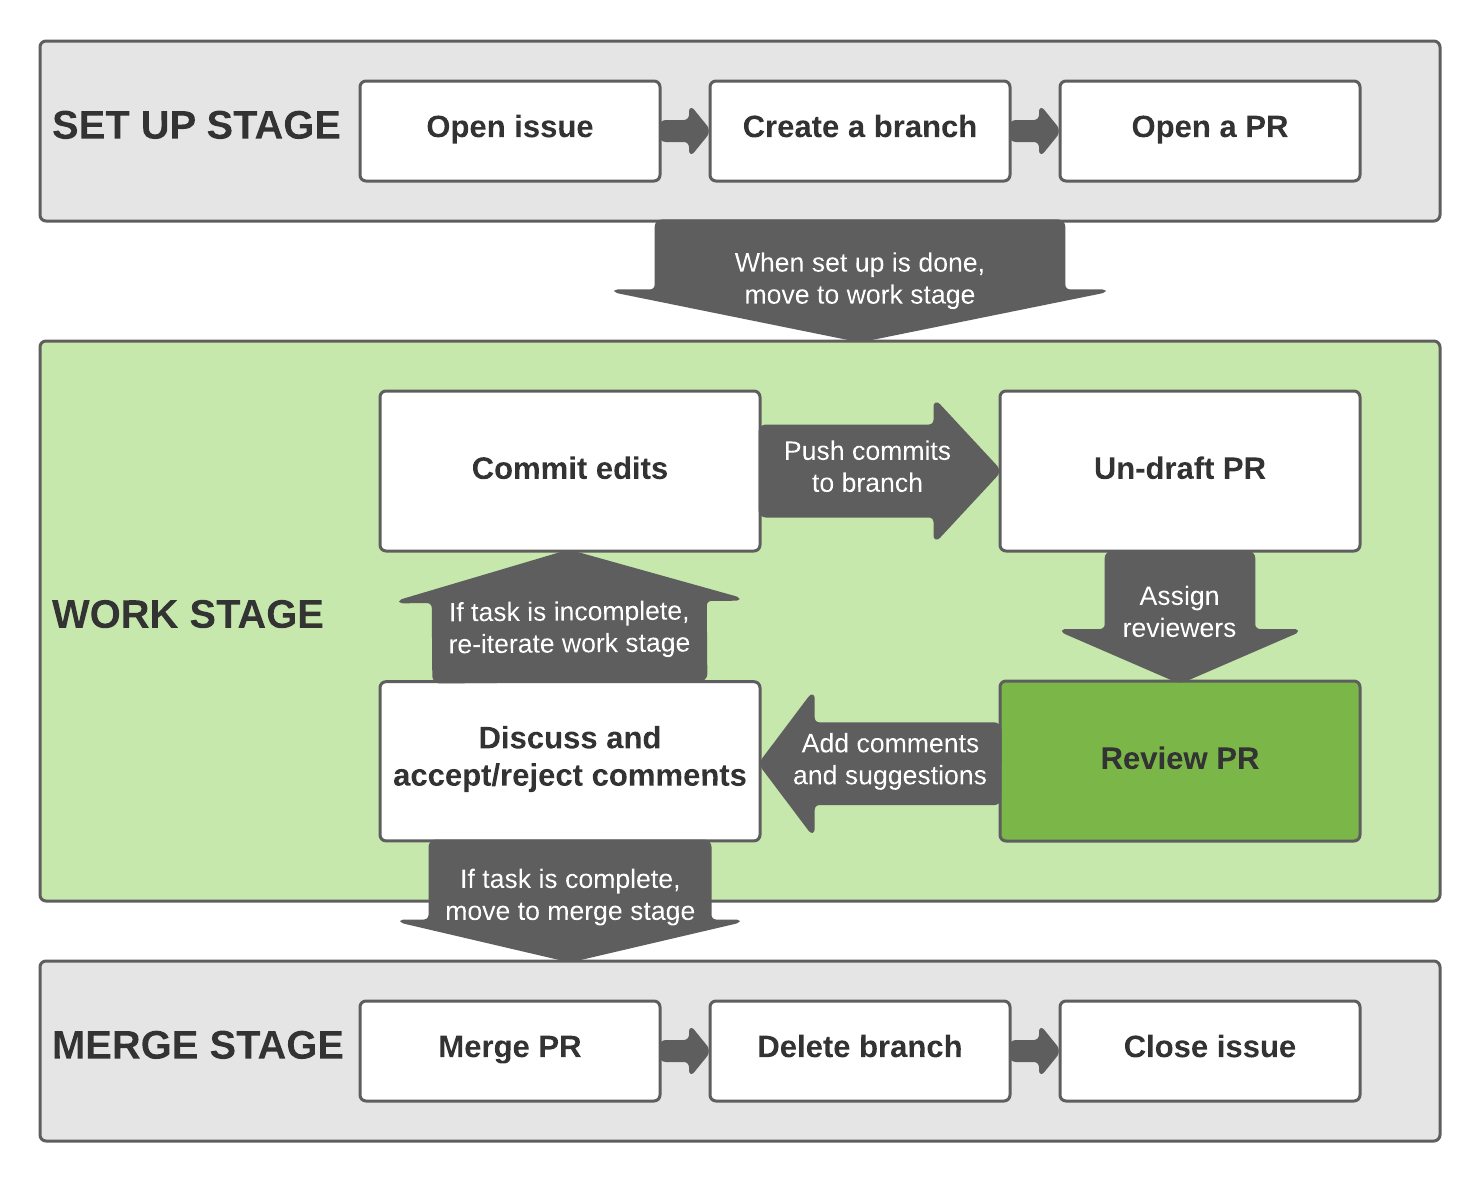
\includegraphics[width=\textwidth]{./img/branch-pr-merge-cycle-S2-3.png}
\end{frame}

\begin{frame}
	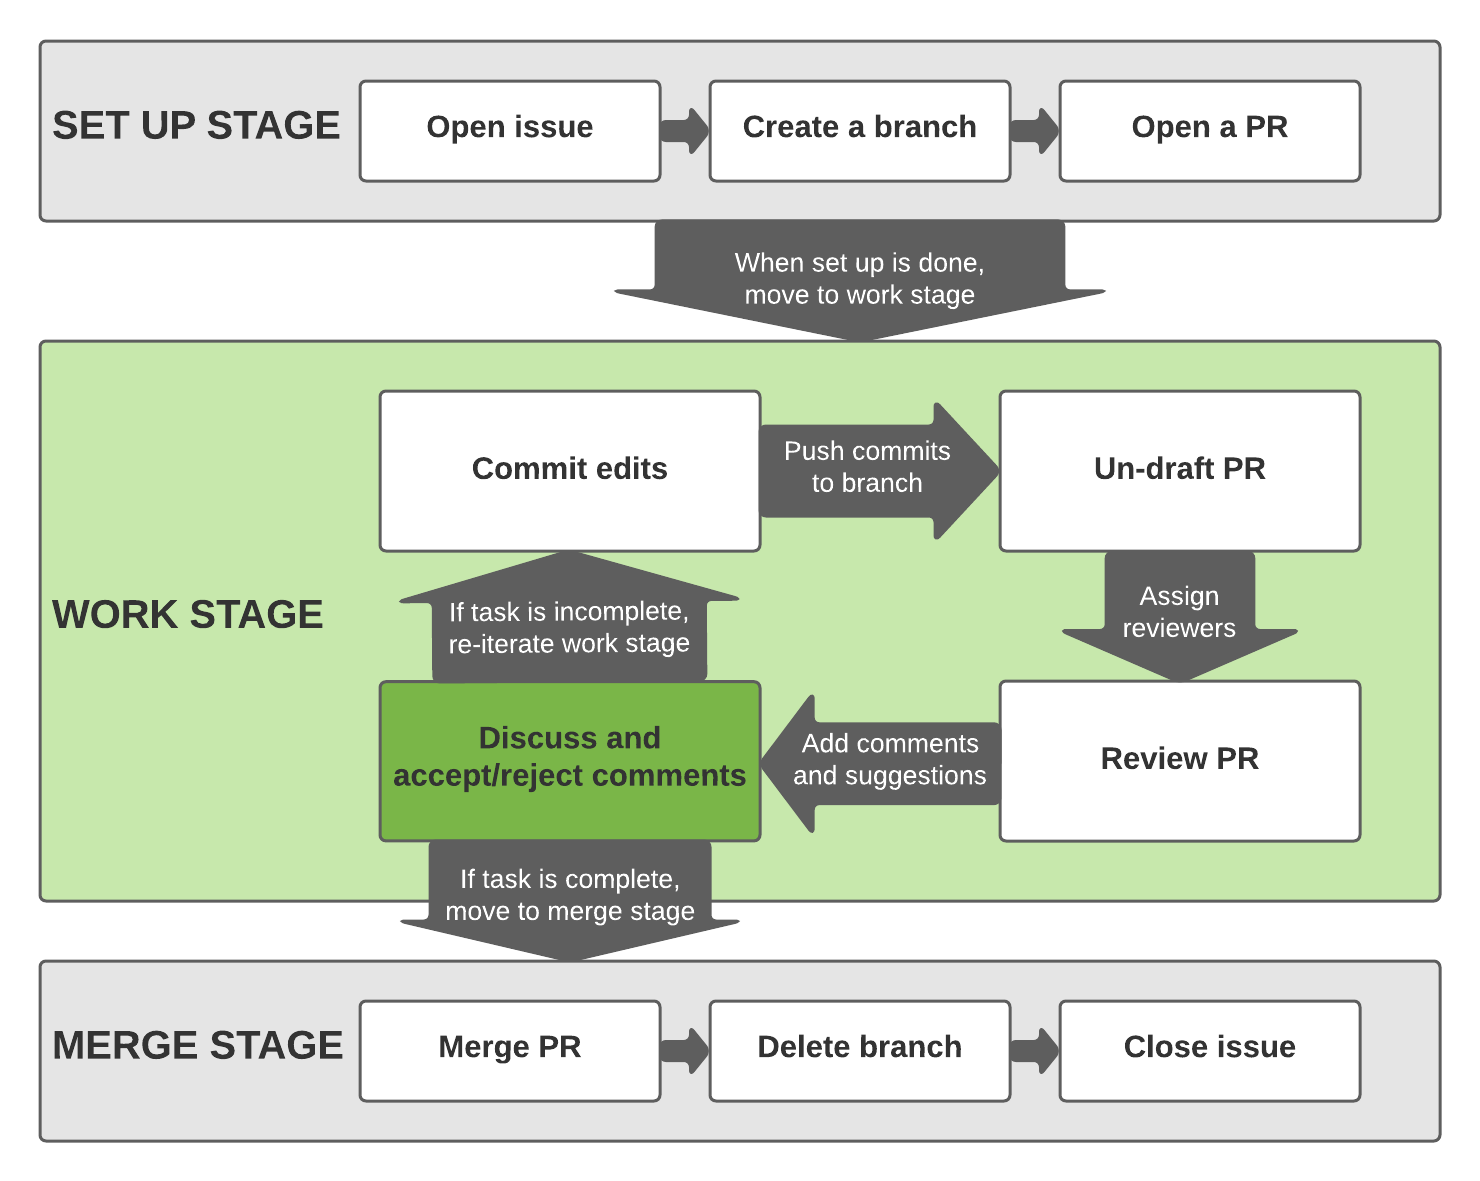
\includegraphics[width=\textwidth]{./img/branch-pr-merge-cycle-S2-4.png}
\end{frame}

\begin{frame}
	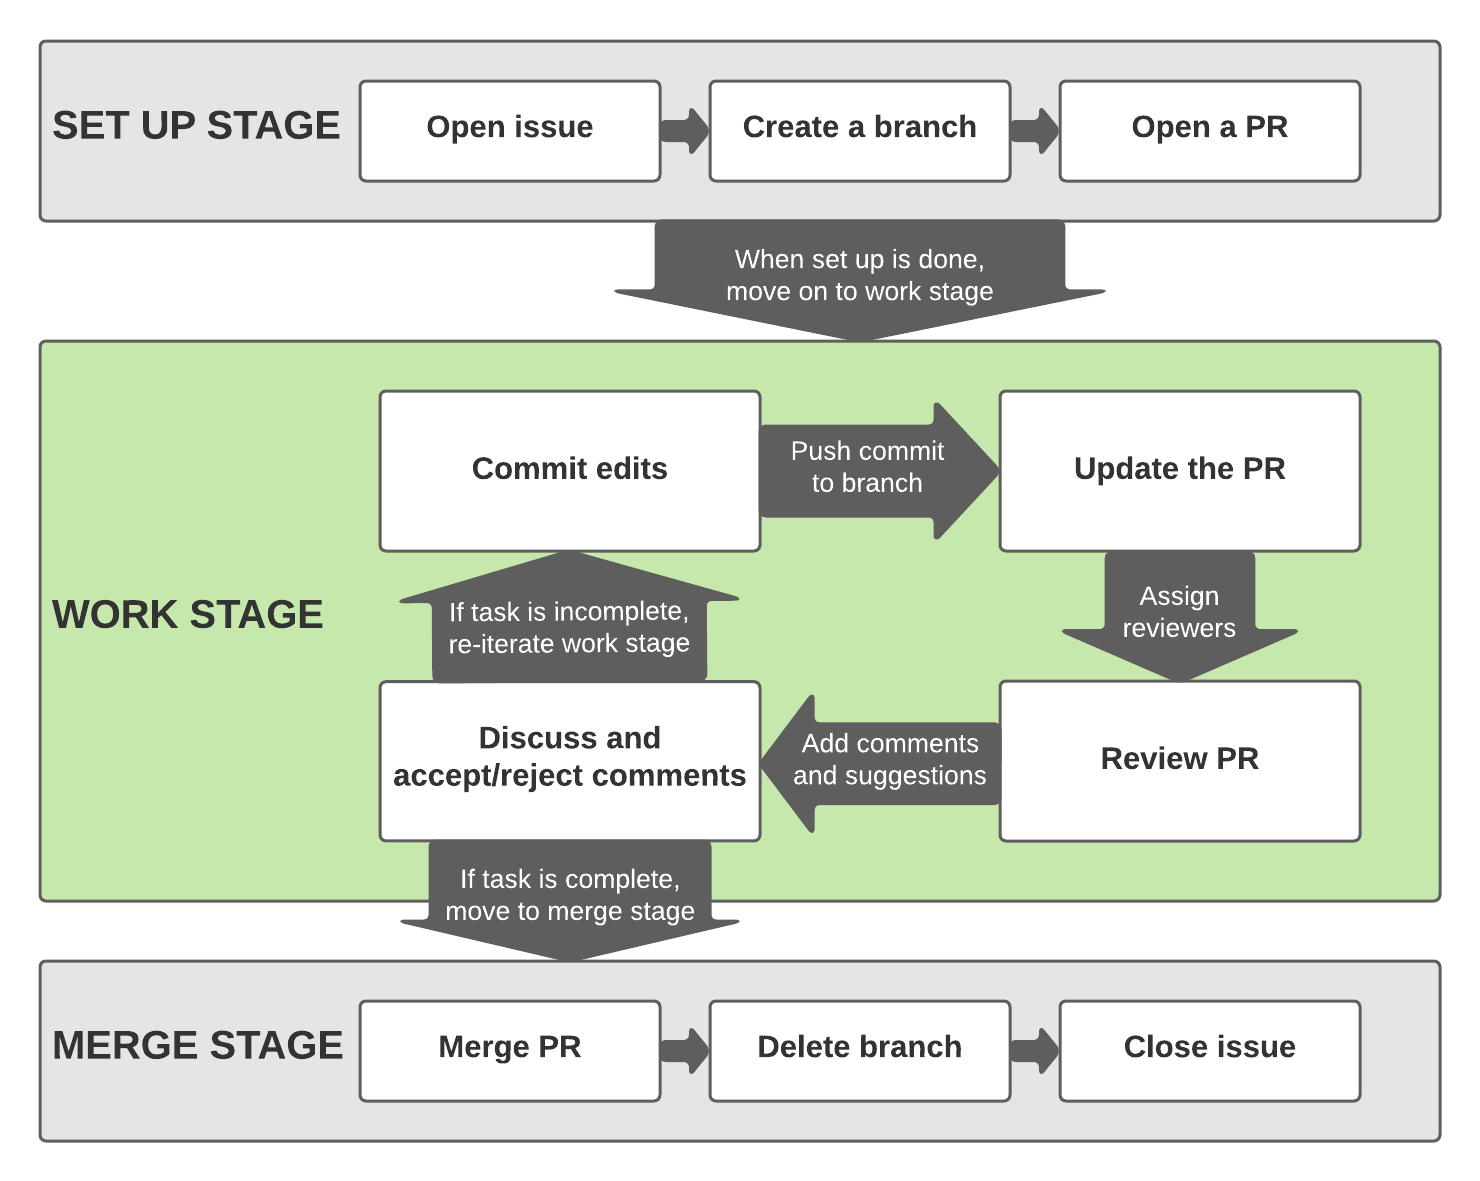
\includegraphics[width=\textwidth]{./img/branch-pr-merge-cycle-S2.png}
\end{frame}

\begin{frame}
	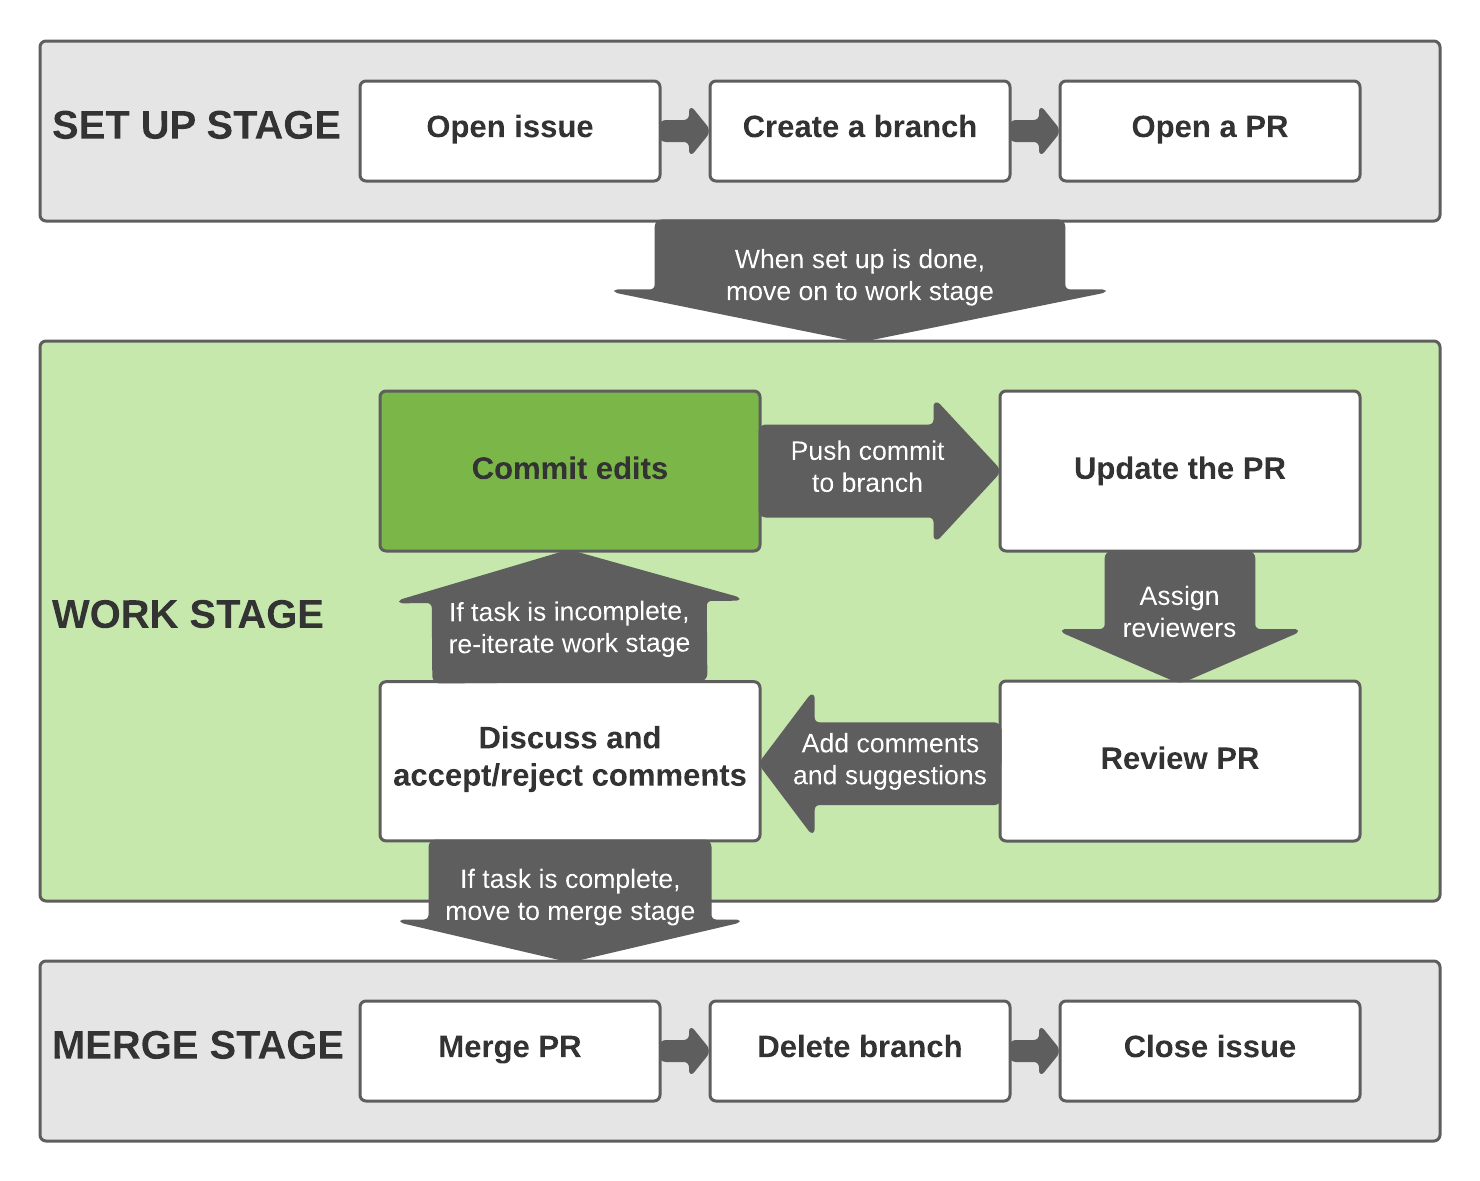
\includegraphics[width=\textwidth]{./img/branch-pr-merge-cycle-S2-1.png}
\end{frame}

\begin{frame}
	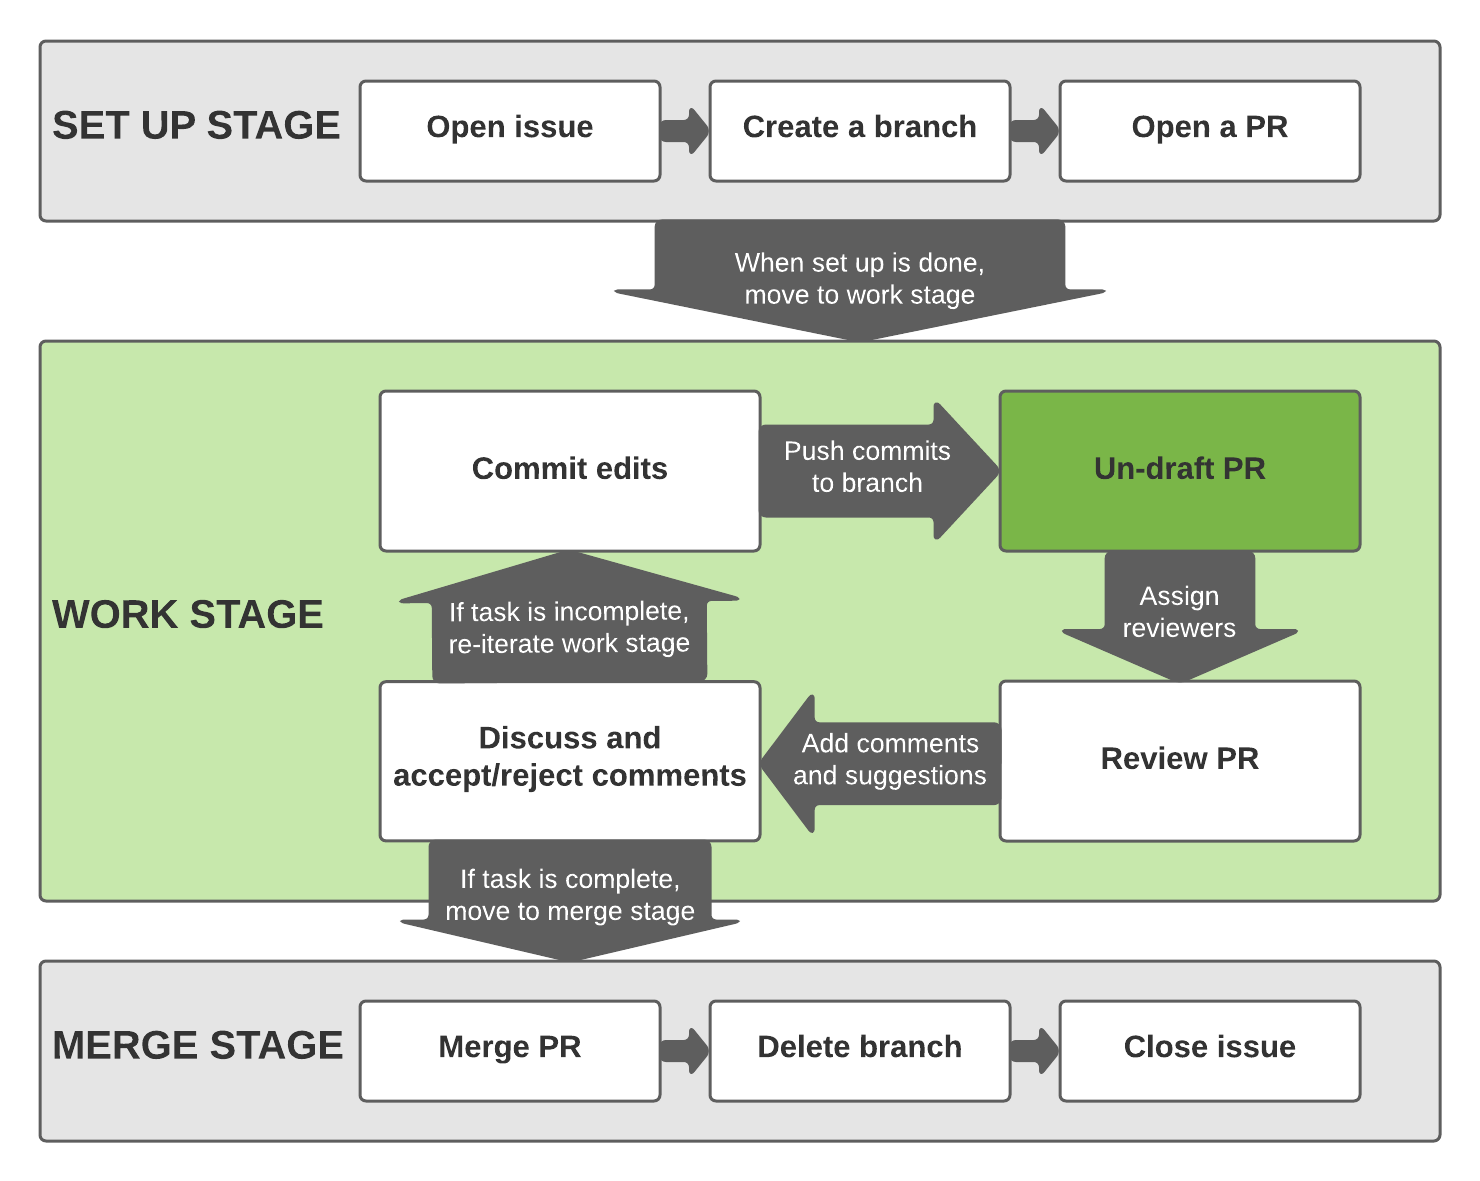
\includegraphics[width=\textwidth]{./img/branch-pr-merge-cycle-S2-2.png}
\end{frame}

\begin{frame}
	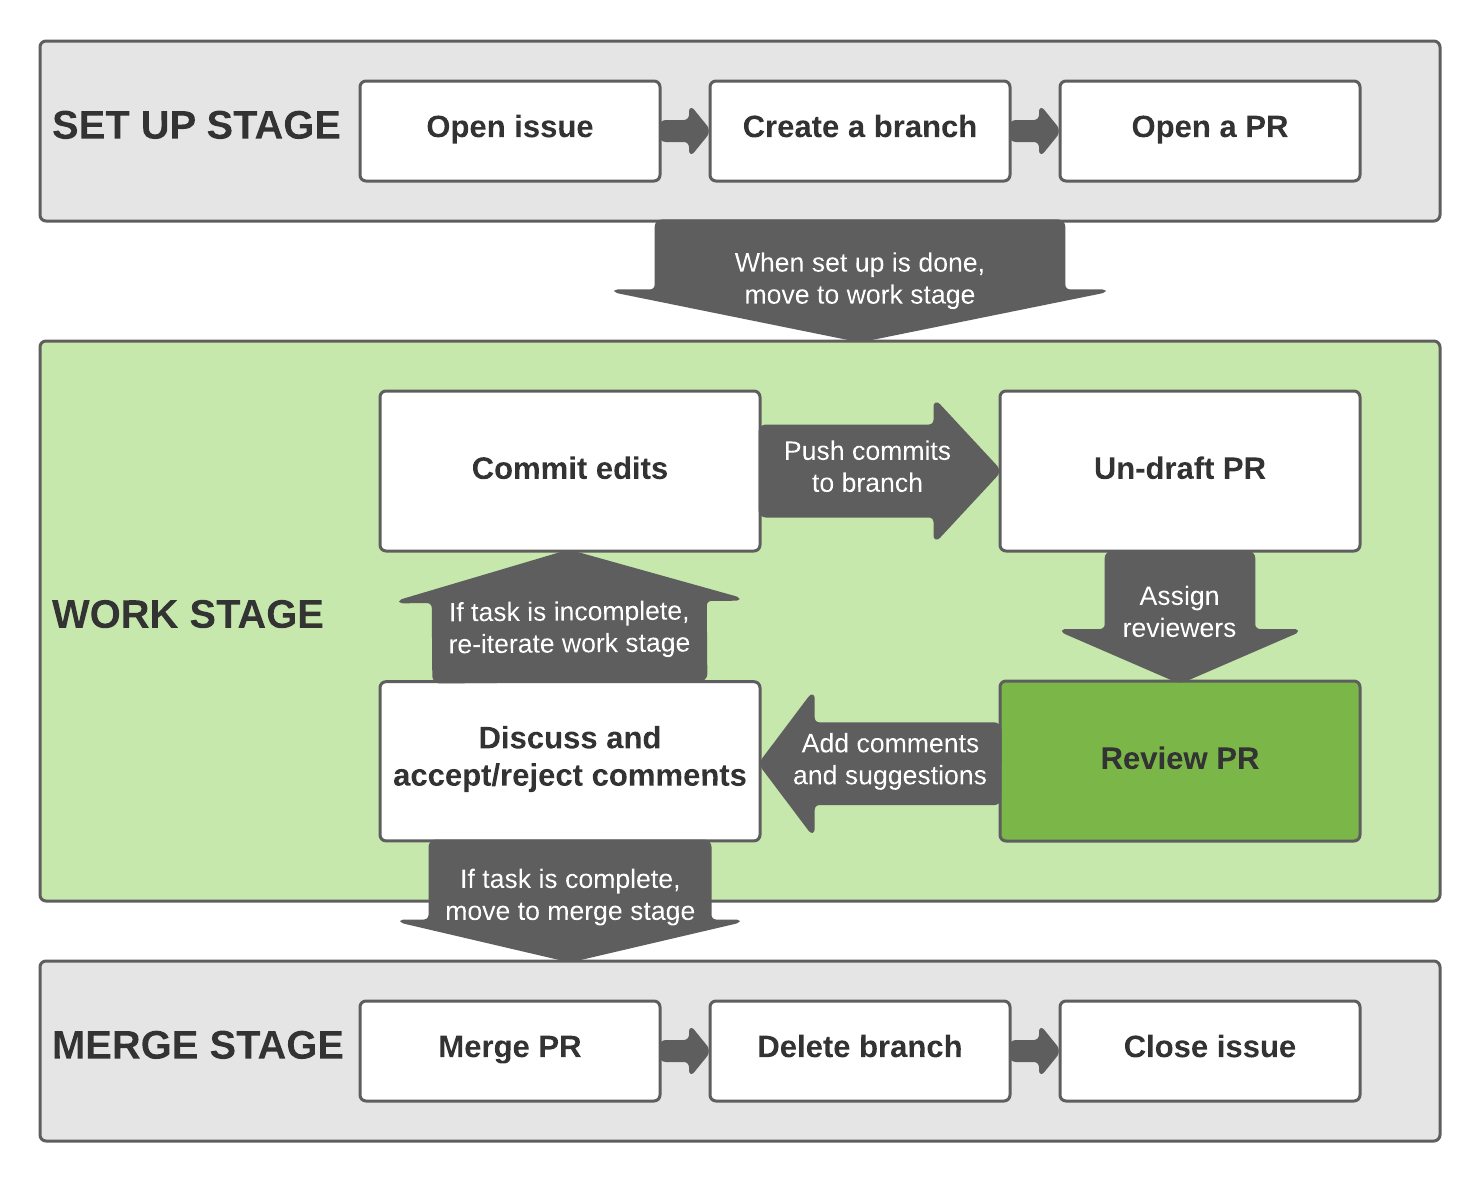
\includegraphics[width=\textwidth]{./img/branch-pr-merge-cycle-S2-3.png}
\end{frame}



\section{Part 2: \newline How to fit the "branch-PR-merge" cycle into your workflow}


\begin{frame}{Useful links}
	\begin{itemize}
	  \item All DIME Analytics GitHub trainings: \trainingURL{https://osf.io/e54gy/}
	  \item Other DIME Analytics GitHub resources: \trainingURL{https://github.com/worldbank/dime-github-trainings}. For example:
		\begin{itemize}
			\item DIME Analytics GitHub Templates (for example .gitignore): \trainingURL{https://github.com/worldbank/dime-github-trainings/tree/master/GitHub-resources/DIME-GitHub-Templates}
			\item DIME Analytics GitHub Roles: \trainingURL{https://github.com/worldbank/dime-github-trainings/blob/master/GitHub-resources/DIME-GitHub-Roles/DIME-GitHub-roles.md}
		\end{itemize}
		\item Markdown cheat sheet (how to format text on GitHub.com):  \trainingURL{https://www.markdownguide.org/cheat-sheet/}
		\item DIME GitHub Account admin info and instructions: \trainingURL{https://github.com/dime-worldbank/dime-account-admin}
	\end{itemize}
\end{frame}


\input{../../Common-Resources/slides/GitHub-Commit-URL.tex}


\end{document}
